\begin{figure}[ht]
	\centering
	\begin{subfigure}[t]{.4825\textwidth}
		\vspace*{\fill}
		\centering
		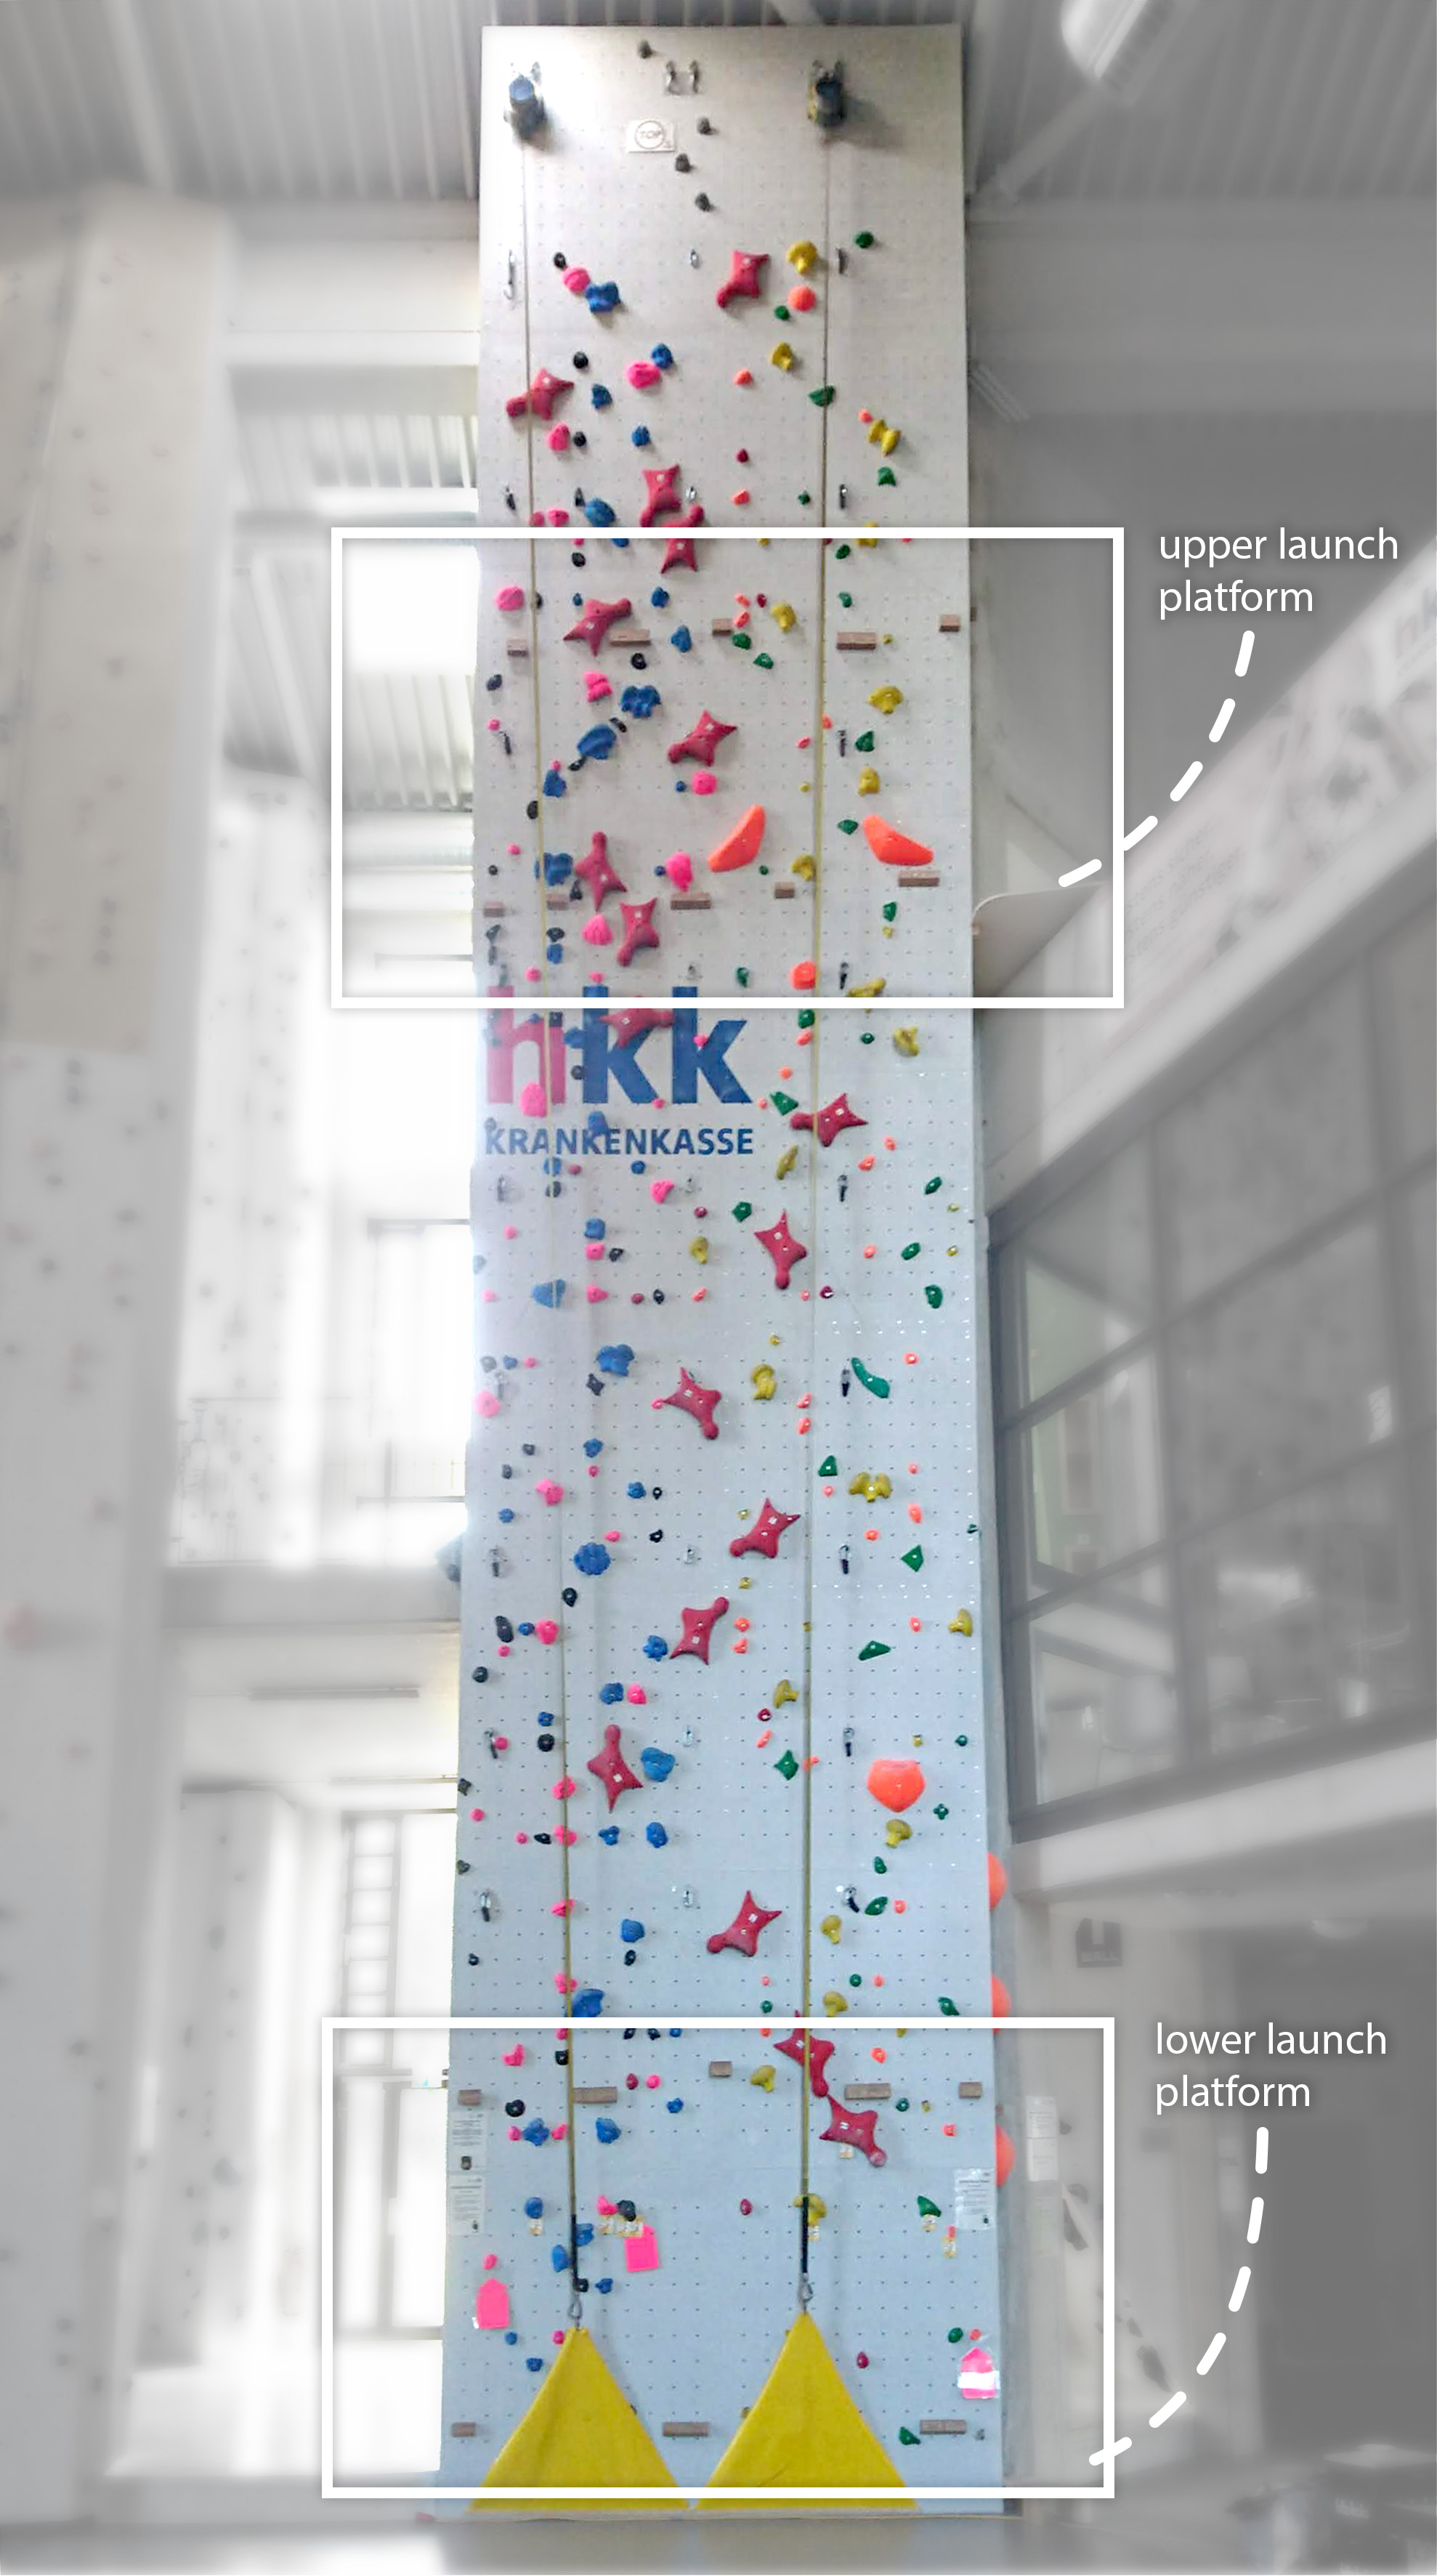
\includegraphics[width=\textwidth]{include/images/climbing-wall-photo.jpg}
		\subcaption{Total view of the \gls{IFSC} lane}
		\label{fig:climbing-wall-photo}
	\end{subfigure}%
	\hfill
	\begin{subfigure}[t]{.48\textwidth}
		\vspace*{\fill}
		\centering
		\hspace*{-0.8cm}
		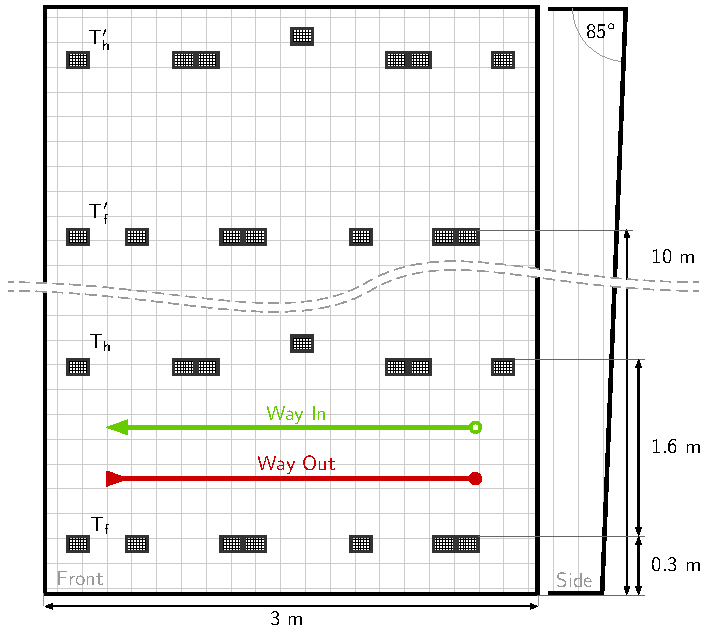
\includegraphics[width=\textwidth]{include/images/climbing-wall-schema.pdf}
		\subcaption{Schematic view of the traversal routes}
		\label{fig:climbing-wall-schema}
		\par\vspace*{0.25cm}
		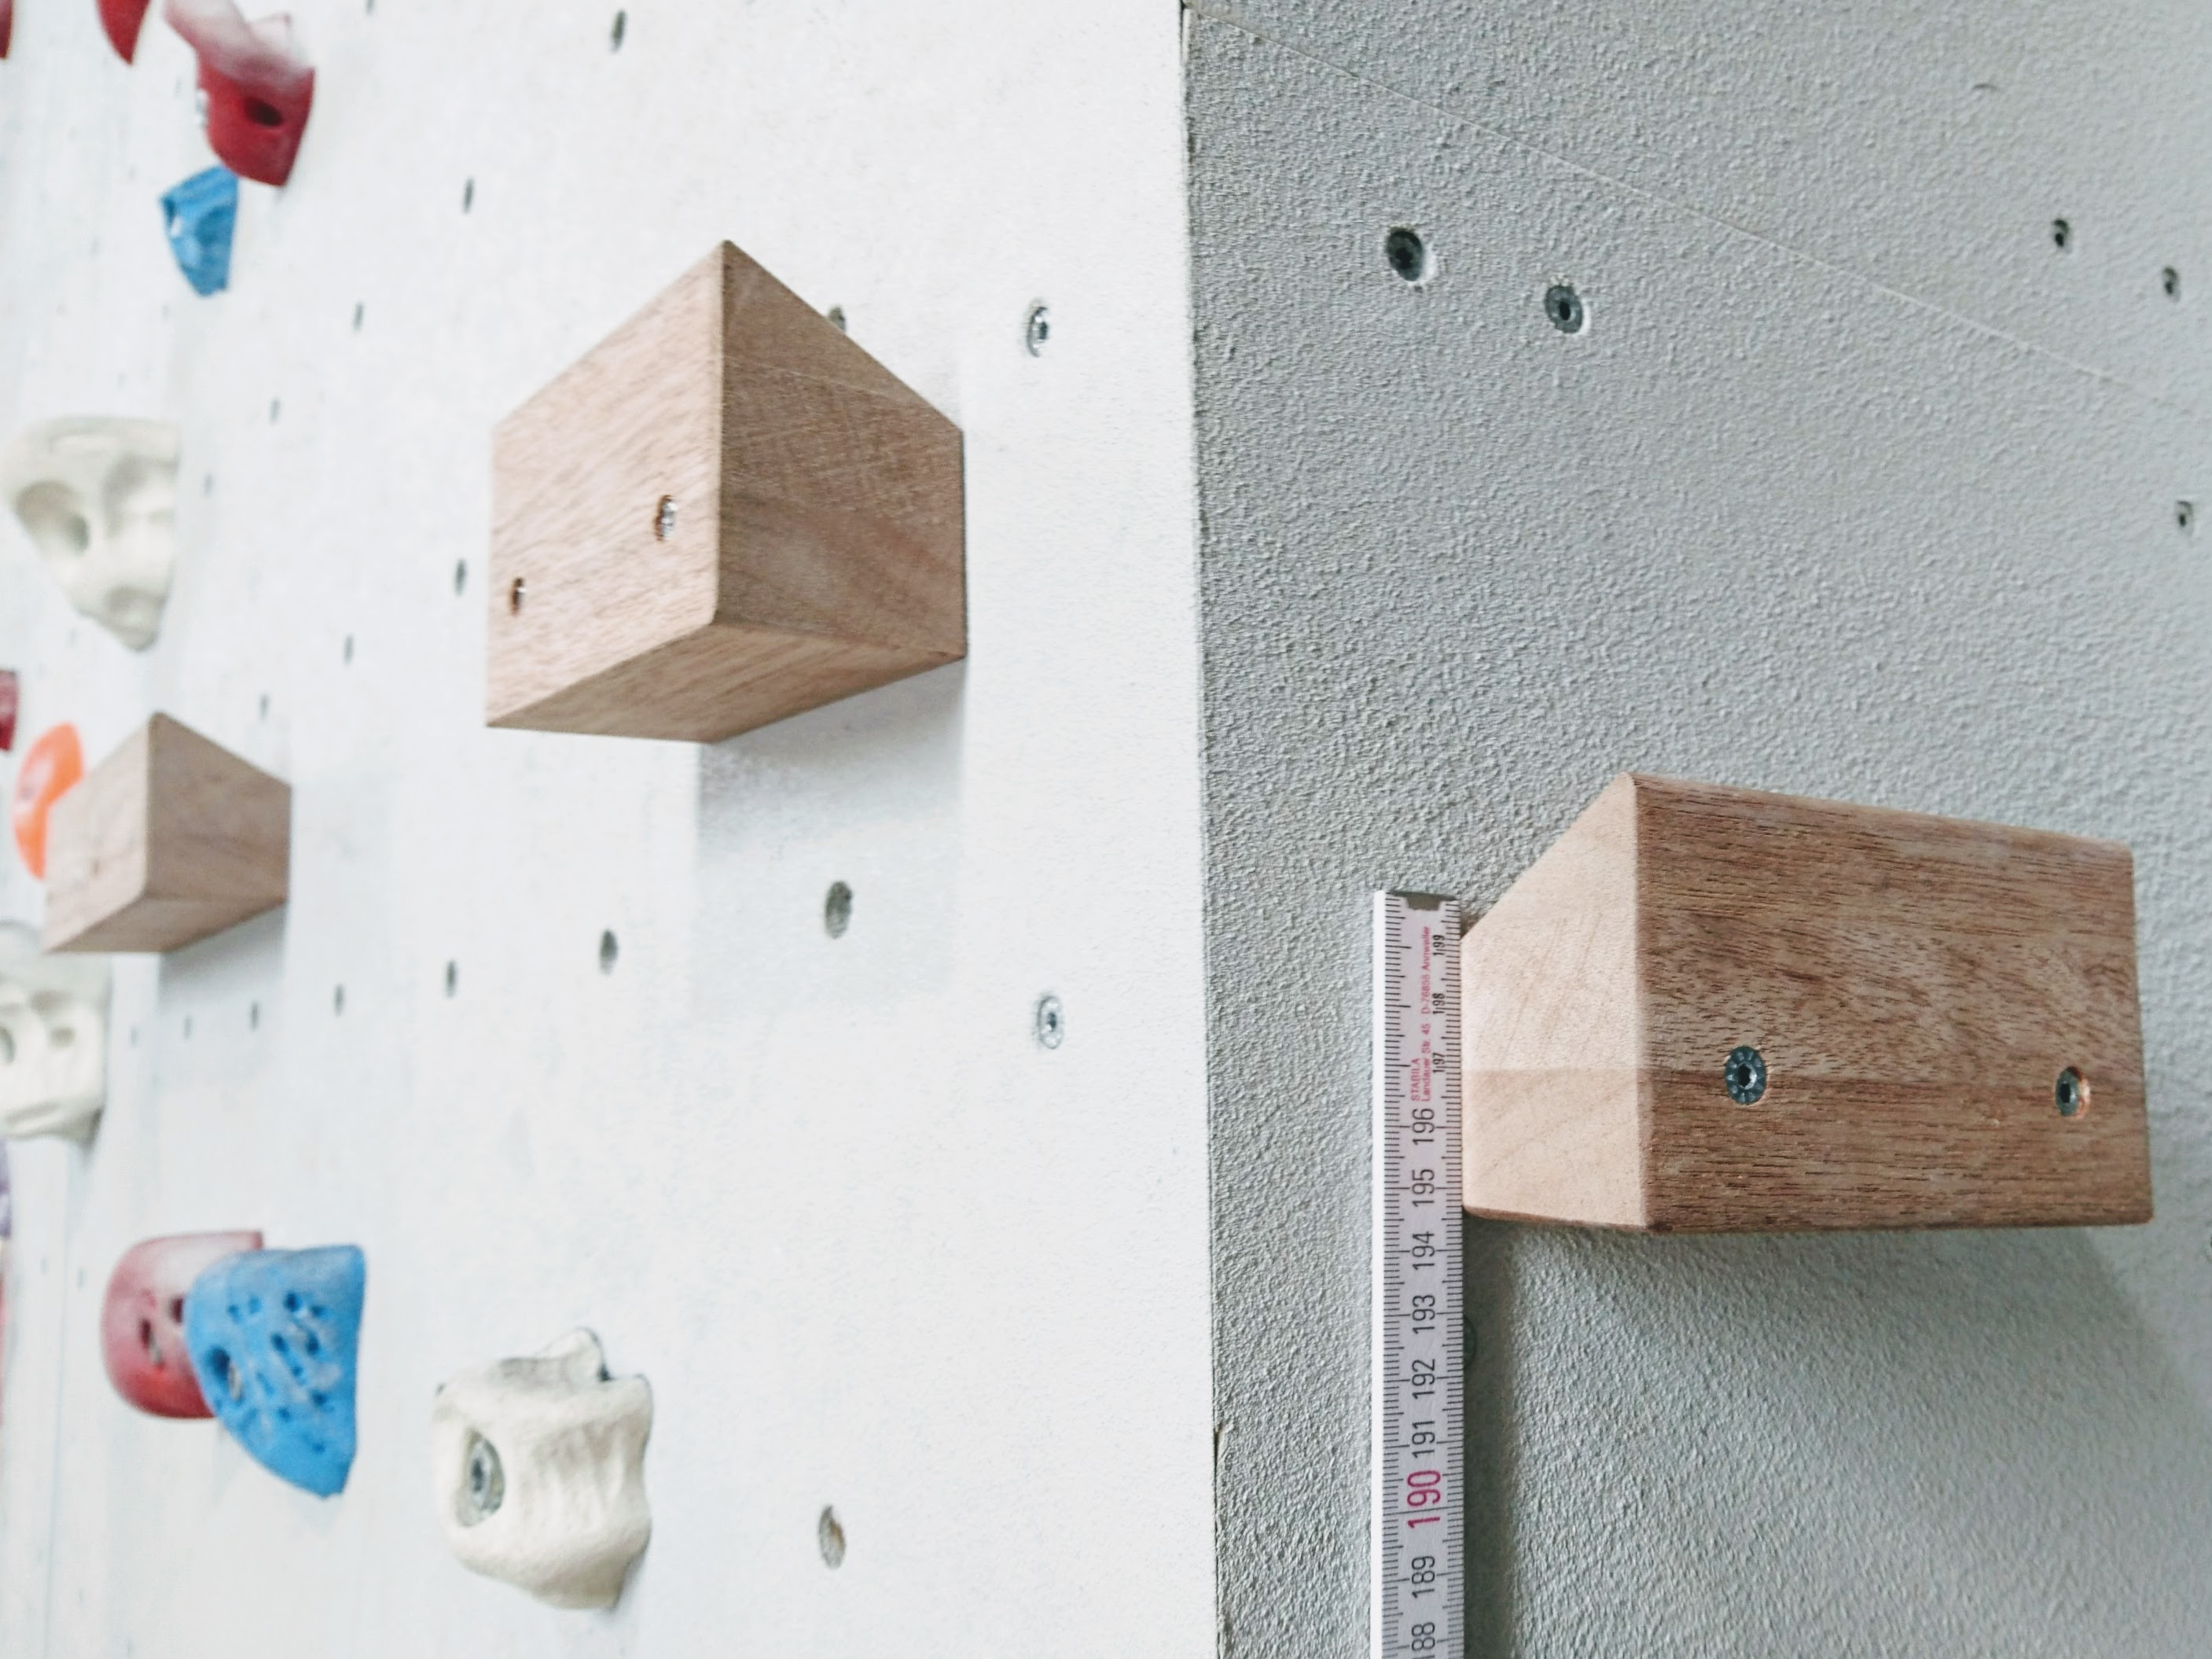
\includegraphics[width=\textwidth]{include/images/hold-photo.jpg}
		\subcaption{Hand holds (w: \SI{12}{\cm}, h: \SI{4/6}{\cm}, d: \SI{4}{\cm})}
		\label{fig:hold-photo}
	\end{subfigure}
	\captionsetup{subrefformat=parens}
	\caption[Climbing routes]{Two identical traversal routes at different heights \subref{fig:climbing-wall-schema}, each consisting of 14 hand and footholds made from wood \subref{fig:hold-photo}; T\textsubscript{h/f} mark the holds at the turning point}
	\label{fig:holds}
\end{figure}